\begin{enumerate}[a)]
	\item En general se usa lo siguiente:
			\begin{align*}
				& \text{Max} \quad x = L_{x}^{0.25}K_{x}^{0.25}\\
				& \begin{array}{ll}
					\text{s.a} & y = L_{y}^{0.5}K_{y}^{0.5}\\[0.2cm]
							   & 25 = L_x + L_y\\[0.2cm]
							   & 25 = K_x + L_y
				  \end{array}
			\end{align*}
		  Por la condición de eficiencia:
		  	$$
		  	\left. 
			  	\begin{array}{c}
					\frac{K_x}{L_x} = \frac{K_y}{L_y}\\
					L_y = 25 - L_x\\
					K_y = 25 - K_x\\
			  	\end{array} 
	  		\right\rbrace \Longrightarrow \frac{K_x}{L_x} = \frac{25 - K_x}{25 - L_x}
		  	$$
		   Siendo las curvas de contrato:
		   	$$K_x = L_x \quad \text{o} \quad K_y = L_y$$
		   	
		   	\begin{center}
		   		\begin{tikzpicture}
		   			% Curva de contrato
		   				\draw[purple] (0,0) -- (4,4);
		   			% Caja
			   			\draw[<->] (0,4.5) node[align=center, above, scale=0.8] {$K_x$} -- (0,0) node[below left] {\footnotesize $O_x$} -- (4.5,0) node[align=center, right, scale=0.8] {$L_x$};
			   			\draw[<->] (-0.5,4) node[align=center, left, scale=0.8] {$L_y$} -- (4,4) node[align=center, above right, scale=0.8] {$O_y$} -- (4,-0.5) node[align=center, below, scale=0.8] {$K_y$};
		   		\end{tikzpicture}
		   	\end{center}
	\item Factores de producción de función de los bienes producidos. En este caso usamos $L$.
			\begin{align*}
				& L_x = K_x \rightarrow x = \left( L_x K_x\right)^{\frac{1}{4}} \rightarrow x = L_x^{\frac{1}{2}} \rightarrow L_x= x^2\\
				& L_y = K_y \rightarrow y = \left( L_y K_y\right)^{\frac{1}{4}} \rightarrow y = L_y^{\frac{1}{2}} \rightarrow L_y= y
			\end{align*}
		  En la restricción de factibilidad
		  	$$L_x + L_y = \overline{L} \rightarrow x^2+y=25 $$
		  Despejando $\textbf{y}$ obtenemos la FPP
		  	$$\therefore y = 25 - x^2$$
		  	\begin{center}
			  	\begin{tikzpicture}
			  		% FPP
				  		% Ejes
					  		\draw[->] (10,0)-- (10,5) node[align=center, above] {\footnotesize $y$};
					  		\draw[->] (10,0) -- (15,0) node[align=center, right] {\footnotesize $x$};
				  		% Curva
				  			\draw [orange] (10,4.5) ..controls (13,3.5) and (14,2.5) .. (14.5,0);
			  		
				  	% Puntos
				  		\draw[black, fill=black] (13.29,2.7) circle[radius=0.05];

			  		% Pendientes
				  		\draw (11.27,4.99) -- (14.68,1.13);
			  	
			  		% Símbolo de paraleleas
				  		\draw (12.19,3.8) -- (12.34,3.93);
				  		\draw (12.24,3.75) -- (12.38,3.88);
			  	\end{tikzpicture}
		  	\end{center}
	\item En general:
				$$
					\begin{array}{ccc}
						\text{Max } U = U\left( x,y\right) & \rightarrow & \text{Max } U = xy\\[0.3cm]
						\text{s.a: } (x,y) \in FPP & \rightarrow & \text{s.a: } y = 25 -x^2
					\end{array}
				$$
		  como las preferencias del consumidor y la tecnología de las empresas son regulares, entonces:
		  		$$	\left\{
						  \begin{array}{l}
						  	 RMS = RMT \Rightarrow \frac{y}{x} = 2x \rightarrow y = 2x^2\\ [.5cm]
						  	 (x,y) \in FPP \Rightarrow y = 25 - x^2
						  \end{array}
					 \right.
		  		$$
		  Finalmente las asignaciones OP son:
		  			q$$\therefore x^{OP} = \frac{25}{3} \approx 2.9 \quad , \quad y^{OP} = \frac{50}{3} \approx 16.7$$
	\item A partir de las asignaciones OP se obtienen:
			$$K_x = l_x = 2.9^2 = 8.4 \quad , \quad K_y = L_y = 16.7$$
		  En el Equilibrio General Competitivo o Walrasiano, a partir de las siguientes expresiones se obtiene toda información:
		  	\begin{itemize}
		  		\item El bien numerario, suele tener como $p =1$ en uno de lo bienes. Por simplicidad, será $p_y = 1$
		  		\item Eficiencia Económica en $L_y$ \footnote{Se es indiferente entre usar $L_y$ o $L_x$}: $PMg_{L_y} = \frac{w}{p_y}$
		  		\item Eficiencia Económica en $K_y$ \footnote{Se es indiferente entre usar $K_y$ o $K_x$}: $PMg_{K_y} = \frac{r}{p_y}$
		  		\item $(x,y) \in FPP$
		  		\item Equilibrio competitivo: $RMS = \frac{p_X}{p_y} = RMT$
		  	\end{itemize}
	  	  Gráficamente:
			\begin{center}
				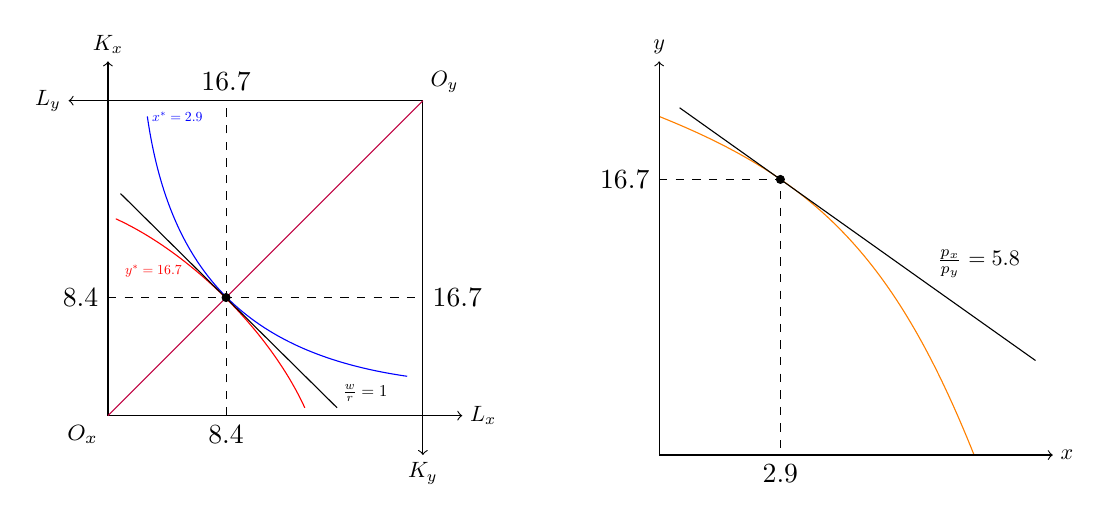
\begin{tikzpicture}
					% Caja en producción
						% Caja
							\draw[<->] (0,4.5) node[align=center, above, scale=0.8] {$K_x$} -- (0,0) node[below left] {\footnotesize $O_x$} -- (4.5,0) node[align=center, right, scale=0.8] {$L_x$};
							\draw[<->] (-0.5,4) node[align=center, left, scale=0.8] {$L_y$} -- (4,4) node[align=center, above right, scale=0.8] {$O_y$} -- (4,-0.5) node[align=center, below, scale=0.8] {$K_y$};
							
						% Dotaciones
							\draw[dashed] (1.5,0) node[below] {8.4} -- (1.5,4) node[above]{16.7};
							\draw[dashed] (0,1.5) node[left] {8.4} -- (4,1.5) node[right]{16.7};
						
						% Curva de contrato
							\draw[purple] (0,0) -- (4,4);
						
						% Cruvas de indiferencia
							\draw [blue] (0.5,3.8) node [right, scale=0.5] {$x^*=2.9$} .. controls (0.79,1.79) and (1.79,0.79) .. (3.8,0.5);
							
							\draw [red] (0.1,2.5)  .. controls (1.06,2.06)  and (2.06,1.06) .. (2.5,0.1);
							\draw [red] (1,1.7) node [above left, scale=0.5] {$y^*=16.7$};
						
						% Pendiente
							\draw[black, fill=black] (1.5,1.5) circle[radius=0.05];
							\draw (0.16,2.82) -- (2.91,0.1) node [above right, scale=0.6] {$\frac{w}{r} = 1$};
						
					% FPP
						% Curva
						\draw [orange] (7,3.8) ..controls (9,3) and (10,2) .. (11,-0.5);
						% Ejes
						\draw [<->] (7,4.5) node[align=center, above, scale=0.8] {$y$} -- (7,-0.5) -- (12,-0.5) node[align=center, right, scale=0.8] {$x$};
						% Recursos
						\draw[dashed] (7,3) node[left] {16.7} -- (8.54,3) -- (8.54,-0.5) node[below]{2.9};
						% Punto
						\draw[black, fill=black] (8.54,3) circle[radius=0.05];
						% Pendiente
						\draw (7.26,3.91) -- (10.44,1.65) node[above right, scale = 0.8] {$\frac{p_x}{p_y} = 5.8$} -- (11.78,0.7);
				\end{tikzpicture}
			\end{center}
\end{enumerate}